\documentclass{beamer}
\mode<presentation>
\usepackage[utf8]{inputenc}

\usetheme{Luebeck}
\usecolortheme{dolphin}
\setbeamertemplate{footline}[frame number]
\setbeamertemplate{caption}[numbered]
\setbeamertemplate{navigation symbols}{}
\setbeameroption{hide notes}
\setbeamertemplate{note page}[plain]
\usepackage[english]{babel}%Set language as english%
\usepackage[babel]{csquotes}%Nicer quotations%
\usepackage{indentfirst}
\usepackage[protrusion=true,expansion=true]{microtype}
\usepackage{enumitem}%Different enumeration options%
%Math Formatting%
\usepackage{amsmath}%AMS Math%
\usepackage{amsthm}%Theorem Formatting%
\usepackage{amssymb}%AMS Symbols%
\usepackage{array}%Allows for more complex matrices
\usepackage{siunitx}%Formats SI units%
\DeclareSIUnit{\molar}{M}%Adds molarity as unit%
\usepackage{booktabs}%Typsets tables%
\newcommand{\specialcell}[2][c]{\begin{tabular}[#1]{@{}l@{}}#2\end{tabular}}
\newcommand{\specialcellbold}[2][c]{%
	\bfseries
	\begin{tabular}[#1]{@{}l@{}}#2\end{tabular}%
}
\usepackage{chemformula}%Typsets Chemical Formulas$
%Image Formatting%
\usepackage{graphicx}%Enchanced graphics support%
\usepackage{media9}
\graphicspath{{./figures/}}
\usepackage{float}%Float options$

\usepackage[
backend=biber,
style=chem-acs
]{biblatex}
\addbibresource{references.bib}

\title{Application of Mathematical Methods in the Study of Chemical Dynamical Systems to an Inventory Multiplier-Accelerator Business Cycle Model}
\author{Benjamin Bui}
\date{May 3, 2019}
\begin{document}
\begin{frame}
	\titlepage
\end{frame}

\section{Introduction}
\begin{frame}{Motivation}
	\begin{columns}
	\begin{column}{0.5\textwidth}
	\begin{itemize}
		\item The study of stochastic processes was deeply influential in explaining macroscale themodynamic properties

		\item Fractals and chaotic processes are a more recent addition to the chemist's toolkit\autocite{Beutel2007,Morris2010}
	\end{itemize}
	\end{column}
	\begin{column}{0.5\textwidth}
		\begin{figure}
			\centering
			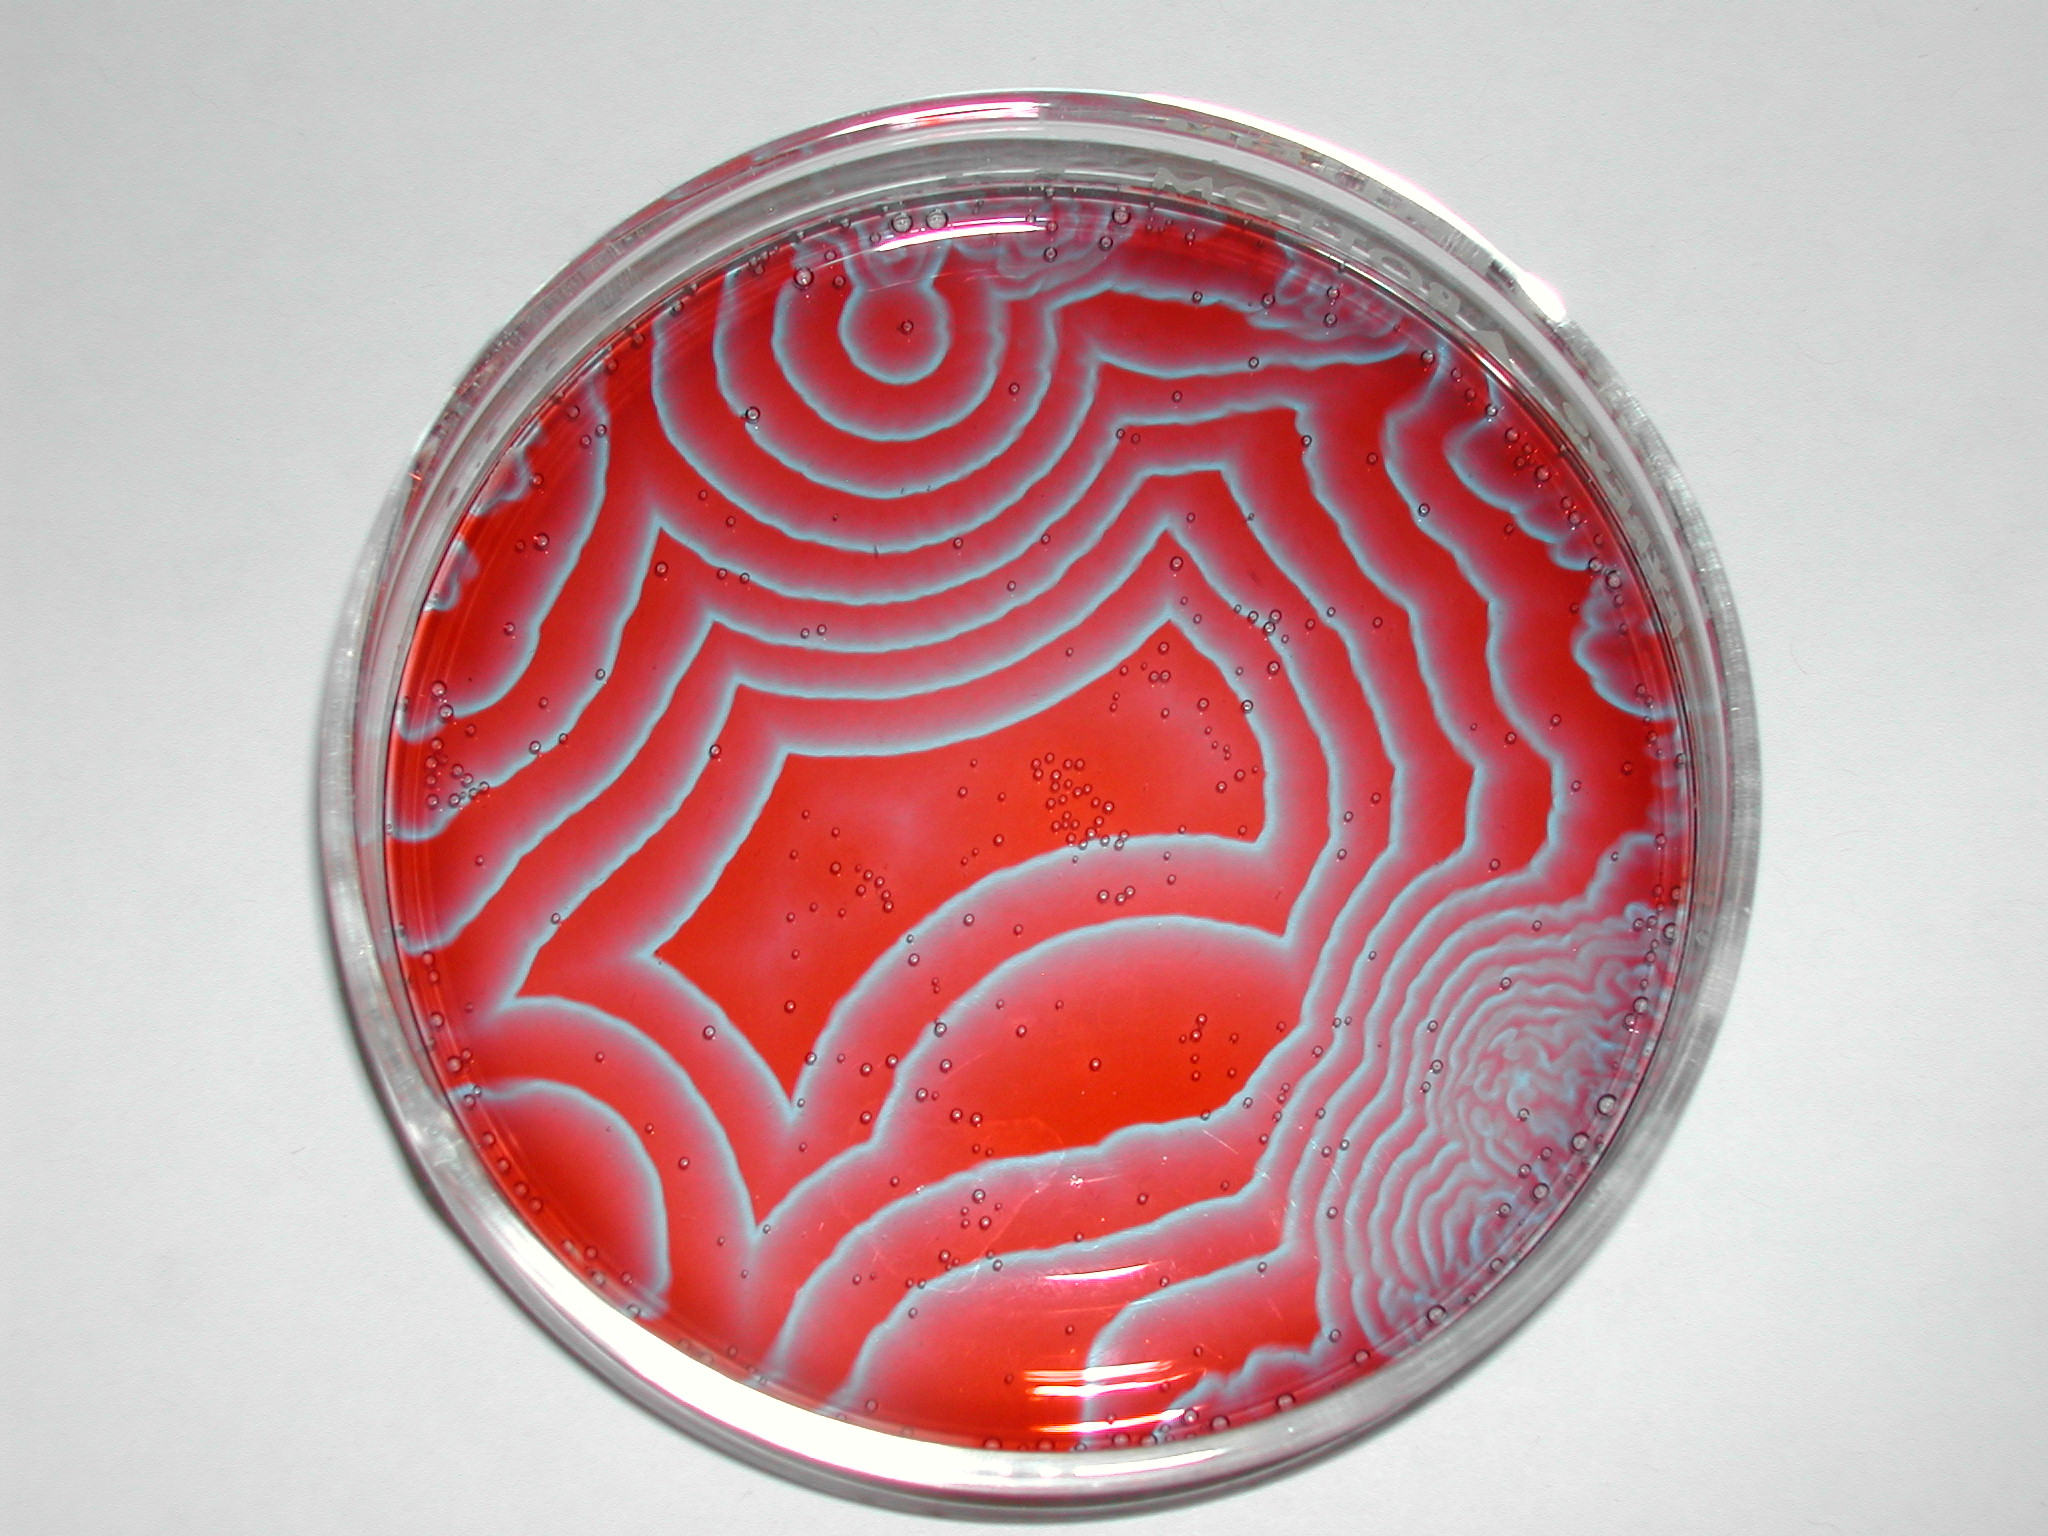
\includegraphics{bz_reaction.jpg}
		\end{figure}
	\end{column}
	\end{columns}
\end{frame}
\note{Test}

\begin{frame}[allowframebreaks]{References}
	\printbibliography
\end{frame}
\end{document}
